
\todo{intro}
\todo{links}
\subsection{The LSTS toolchain}
    The Underwater Systems and Technology Laboratory of Porto university offers an extensive toolchain for the control and operation of unmanned air, ground and surface vehicles. This thesis has used the Neptus-IMC-Dune software toolchain shown in figure \ref{fig:lsts-toolchain}.
    
    \begin{figure}[!htbp]
        \centering
        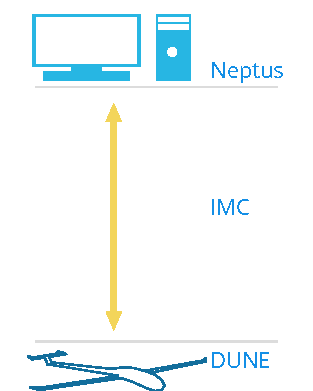
\includegraphics{bilder/lsts-toolchain.pdf}
        \caption{The Neptus-IMC-Dune toolchain}
        \label{fig:lsts-toolchain}
    \end{figure}
    \subsubsection{DUNE}
    Dune: Unified Navigation Environment (DUNE) is the software package running on the vehicle, providing a framework for a number of tasks. It is a highly modular thread based system, splitting execution into separate blocks known as \textit{tasks}. Tasks can be responsible for low level operations, such as interaction with sensors and actuators, or complex higher level operations such as plan execution and vehicle supervision. Inter-thread communication is realised through the IMC protocol, where each task can bind itself to any IMC message types and and handle them as desired. Dune focuses on code reuse, offering a large codebase for a number of applications, while also offering scripts for easily creating new tasks, all of which are configured through a set of configuration files. \todo{Include small part about CMake?}
    
    \subsubsection{IMC}
    The Inter-Module Communication (IMC) protocol implements seamless inter- and intra-vehicle communication. It offers custom serialization methods and can therefore transmit data independently of network medium. IMC message types are generated from and described in an xml file.
    
    \subsubsection{Neptus}
    Neptus is a command and control software for the operation of all types of vehicles. It serves as an interface between operator and vehicles at ground control for several phases of a mission; planning, simulation, execution and post-mission analysis. It employs the IMC protocol to communicate with platforms running Dune.
    
    \subsubsection{GLUED}
    GNU/Linux Uniform Environment Distribution (GLUED) is a minimal linux distribution designed to run on an embedded system. It is designed to be as lightweight as possible, and is easily updated with cross compiled packages. It is also highly configurable.

\subsection{RTKLIB}
\label{seq:rtklib}
RTKLIB is an open-source program package for GNSS-related operations created by Tomoji Takasu. It supports all currently existing GNSS and some augmentation systems. Various positioning modes are supported and both input and output is configurable to be in the form of a number of different protocols. Further, it contains a substantial code base for positioning operations.